\documentclass{bookSolutions}

\title{Kreyszig  Introductory functional analysis with applications}
\author{Sergio Garrido}

\begin{document}
\maketitle

\tableofcontents

\section{Metric spaces}
\subsection{Metric space}

1 This is of course the most important metric space there is
2 Not so useful counterexample of a metric on R
4 There's infinitely many, but they're all kind of the "same"
5 Shows we can always multiply a metric with a number
6 Very important metric which ends up encoding uniform convergence 
8 Another very useful example of a metric leading eventually to the $L^1$ spaces 
9 The discrete metric is not so important except for counterexamples
11 Useful consequence of the triangle inequality
12 Useful consequence of the triangle inequality
13 Useful consequence of the triangle inequality
15 This one is pretty neat to see how some of the axioms are actually superfluous. Cool but not so important

\begin{exercise}{1}
Show that the real line is a metric space
\end{exercise}
\begin{proof}
fill
\end{proof}

\begin{exercise}{2}
Does $d(x,y)=(x-y)^2$ define a metric on the set of all real numbers?
\end{exercise}
\begin{proof}
fill
\end{proof}

\begin{exercise}{4}
Find all metrics on a set $X$ consisting of two points. Consisting of one point.
\end{exercise}
\begin{proof}
fill
\end{proof}

\begin{exercise}{5}
Let $d$ be a metric of $X$. Determine all constants $k$ such that (i) $kd$, (ii) $d+k$ is a metric on $X$
\end{exercise}
\begin{proof}
fill
\end{proof}

\begin{exercise}{6}
Show that $d$ in 1.1-6 satisfies the triangle inequality.
\end{exercise}
\begin{proof}
fill
\end{proof}

\begin{exercise}{8}
Show that another metric $\tilde{d}$ on the set $X$ in 1.1-7 is defined by $\tilde{d}(x,y)=\int_a^b\absoluteValue{x(t)-y(t)}dt$.
\end{exercise}
\begin{proof}
fill
\end{proof}

\begin{exercise}{9}
Show that $d$ in 1.1-8 is a metric.
\end{exercise}
\begin{proof}
fill
\end{proof}

\begin{exercise}{11}
Prove (1).
\end{exercise}
\begin{proof}
fill
\end{proof}

\begin{exercise}{12 (Triangle inequality)}
The triangle inequality has several useful consequences. For instance, using (1), show that $\absoluteValue{d(x,y)-d(z,w)}\leq d(x,z)+d(y,w)$
\end{exercise}
\begin{proof}
fill
\end{proof}

\begin{exercise}{13}
Using the triangle inequality show that $\absoluteValue{d(x,z)-d(y,z)}\leq d(x,y)$
\end{exercise}
\begin{proof}
fill
\end{proof}

\begin{exercise}{15}
Show that nonnegativity of a metric follows from (M2) to (M4).
\end{exercise}
\begin{proof}
fill
\end{proof}

\subsection{Further examples of metric spaces}


\begin{exercise}{3}
Show that the Cauchy-Schwarz inequality (11) implies 
\[
(\absoluteValue{x_1}+\dots+\absoluteValue{x_n})^2 
\leq n (\absoluteValue{x_1}^2+\dots+\absoluteValue{x_n}^2).
\]
\end{exercise}
\begin{proof}
Consider $(x_1,\dots,x_n)$ and $(1,\dots,1)$, $n$ times. Then the Cauchy-Schwarz inequality tells us
\[
\sum^n_{i=1}\absoluteValue{x_i} \leq
\sqrt{\sum_{i=1}^n\absoluteValue{x_i}^2}\sqrt{\sum_{i=1}^n\absoluteValue{1}^2} 
=\sqrt{\sum_{i=1}^n\absoluteValue{x_i}^2}\sqrt{n}.
\]
Squaring both sides of the inequality gives us the desired result.
\end{proof}

\begin{exercise}{4 (Space $l^p$)}
Find a sequence which converges to 0, but is not in any space $l^p$, where $1\leq p<+\infty$.
\end{exercise}
\begin{proof}
Consider the sequence $x_n=1/\log_2(n)$. This sequence converges to 0 because $\log_2(n)\to\infty$ as $n\to\infty$. However, we can do the Cauchy condensation test on the series $\sum_{n=1}^\infty 1/\absoluteValue{\log_2(n)}^p$ (to see whether $x_n$ is in $l^p$). We have 
\begin{align*}
    \sum_{n=1}^\infty \frac{2^n}{\absoluteValue{\log_2(2^n)}^p} 
    =\sum_{n=1}^\infty \frac{2^n}{\absoluteValue{n}^p}.
\end{align*}
Now using the ratio test on the sequence $2^n/\absoluteValue{n}^p$, we obtain
\[
\lim_{n\to\infty}\frac{2^{n+1}/\absoluteValue{(n+1)}^p}{2^n/\absoluteValue{n}^p} =2,
\]
so that the series does not converge for any $p$, giving us the desired result.
\end{proof}

\begin{exercise}{5}
Find a sequence which is in $l^p$ with $p>1$, but $x\notin l^1$.
\end{exercise}
\begin{proof}
We have that the series associated to the sequence $x_n=1/n$ does not converge for $p=1$ but it does for $p>1$, as required.
\end{proof}

\begin{exercise}{6 (Diameter, bounded set)}
The diameter $\delta(A)$ of a nonempty set $A$ in a metric space $(X,d)$ is defined to be 
\[
\delta(A) =\sup_{x,y\in A}d(x,y).
\]
$A$ is said to be bounded if $\delta(A)<\infty$. Show that $A\subseteq B$ implies $\delta(A)\leq\delta(B)$.
\end{exercise}
\begin{proof}
Since $\delta(B)=\sup{x,y\in B}d(x,y)$, then $\delta(B)$ is an upper bound for all the distances between the elements of $B$. However, because $A\subseteq B$, then the set of distances between the elements of $A$ is a subset of the set of distances between the elements of $B$. Hence $\delta(B)$ is also an upper bound for the set of distances between the elements of $A$. Thus, the least upper bound of such set, namely $\delta(A)$ is less than or equal to any other upper bound of such set, so that $\delta(A)\leq\delta(B)$, as required.
\end{proof}

\begin{exercise}{7}
Show that $\delta(A)=0$ (cf. exercise 6) if and only if $A$ consists of a single point.
\end{exercise}
\begin{proof}
Suppose $\delta(A)$ is 0, then for all $x,y\in A$, $d(x,y)=0$ (because $d$ is nonnegative), since $d(x,y)=0$ if and only if $x=y$, then $A$ consists of a single point. 

Conversely, suppose $A$ consists of a single point. Then $\delta(A) = \sup_{x,y\in A}d(x,y) =0$, as required.
\end{proof}

\begin{exercise}{11}
If $(X,d)$ is any metric space, show that another metric on $X$ is defined by
\[
\hat{d}(x,y)=\frac{d(x,y)}{1+d(x,y)},
\]
and $X$ is bounded in the metric $\hat{d}$.
\end{exercise}
\begin{proof}
M1, M2 and M3 follow directly from the properties of $d$ and the fact that the function $f(t)=t/(1+t)$ defined on the nonnegative reals does not alter these properties.

The proof that M4 holds for $\hat{d}$ is essentially the same as in 1.2-1, which I reproduce here for completeness. We have that $f'(t)=1/(1+t)^2$, which is positive, so that $f(t)$ is monotonically increasing. Thus, if $\absoluteValue{a+b}\leq \absoluteValue{a}+\absoluteValue{b}$, then $f(\absoluteValue{a+b})\leq f(\absoluteValue{a}+\absoluteValue{b})$. Knowing this, we have that 
\begin{align*}
    \frac{\absoluteValue{a+b}}{(1+\absoluteValue{a+b})} \leq& \frac{\absoluteValue{a}+\absoluteValue{b}}{1+\absoluteValue{a}+\absoluteValue{b}}\\
    \leq& \frac{\absoluteValue{a}}{1+\absoluteValue{a}} 
    + \frac{\absoluteValue{b}}{1++\absoluteValue{b}}.
\end{align*}
Replacing $a=d(x,z)$ and $b=d(z,y)$ in the above inequality we get the desired result.

To prove that $X$ is bounded under $\hat{d}$, consider the following two cases.

First: if $X$ is bounded under $d$, then $d(x,y)$ has an upper bound for all $x,y$ so that $\sup_{x,y\in X}\hat{d}(x,y)<\infty$.

Second: if $X$ is not bounded under $d$, then we have to check the limiting process of $\hat{d}$ whenever $d(x,y)\to\infty$ for some $x,y\in X$. In that case, we have $\lim_{d(x,y)\to\infty}\frac{d(x,y)}{1+d(x,y)}=1$, so that $\sup_{x,y\in X}\hat{d}(x,y)\leq \infty$, as required.
\end{proof}

\begin{exercise}{12}
Show that the union of two bounded sets $A$ and $B$ in a metric space is bounded. (Definition in exercise 6).
\end{exercise}
\begin{proof}
Suppose $A$ and $B$ are bounded. Let $a\in A\cup B$ be arbitrary and fix $a_0\in A$ and $b_0\in B$. If both $a_0,b_0$ are in either $A$ or $B$ then they they are bounded because both $A$ and $B$ are bounded. So suppose $a_0\in A$ and $b_0\in B$. By the generalised triangle inequality, with $x_1=a, x_2=a_0, x_3=b_0$ and $x_4=b$ (exercise 1.11), we obtain $d(a,b)\leq d(a,a_0)+d(a_0,b_0)+d(b_0,b)$. The first and the last terms of that inequality are bounded because $A$ and $B$ are bounded. Furthermore, by M1, $d(a_0,b_0)$ is finite. Thus, the right hand side of the inequality has an upper bound and since $a$ and $b$ were chosen arbitrarily, then $A\cup B$ is bounded.
\end{proof}

\begin{exercise}{13 (Product of metric spaces)}
The Cartesian product $X=X_1\times X_2$ of two metric spaces $(X_1, d_1)$ and $(X_2, d_2)$ can be made into a metric space $(X, d)$ in many ways. For instance, show that a metric $d$ is defined by $d(x,y)=d_1(x_1,y_1)+d_2(x_2,y_2)$, where $x=(x_1,x_2)$ and $y=(y_1,y_2)$.
\end{exercise}
\begin{proof}
M1, M2 and M3 follow from the fact that $d$ is an addition and the properties of $d_1$ and $d_2$. To see that M4 holds, let $x,y,z\in X_1\times X_2$. We have $d(x,y) =d_1(x_1,y_1)+d_2(x_2,y_2) \leq d_1(x_1,z_1)+d_1(z_1,y_1) + d_2(x_2,z_2)+d_2(z_2,y_2) = d(x,z)+d(z,y)$, as required.
\end{proof}

\begin{exercise}{14}
Show that another metric on $X_1\times X_2$ (as in exercise 13) is defined by $\hat{d}(x,y)=\sqrt{d_1(x_1,y_1)^2+d_2(x_2,y_2)^2}$.
\end{exercise}
\begin{proof}
M1, M2 and M3 follow directly from the properties of $d_1$ and $d_2$ and the functions that compose them: first squaring, then addition and then taking root, all of which preserve these properties of metrics. To see M4 holds, let $x,y,z\in X_1\times X_2$. We have 
\begin{align*}
    \hat{d}(x,y) =& [d_1(x_1,y_1)^2+d_2(x_2,y_2)^2]^{1/2}\\
    \leq& [[d_1(x_1,z_1)+d_1(z_1,y_1)]^2+[d_2(x_2,z_2)+d_2(z_2,y_2)]^2]^{1/2}\\
    =& [d_1(x_1,z_1)^2+2d_1(x_1,z_1)d_1(z_1,y_1)+d_1(z_1,y_1)^2\\
    &+ d_2(x_2,z_2)^2+2d_2(x_2,z_2)d_2(z_2,y_2)+d_2(z_2,y_2)^2]^{1/2}
\end{align*}
squaring both sides of the inequality, and using the the Cauchy-Schwarz inequality in those terms that contain a factor of 2:
\begin{align*}
    \hat{d}(x,y)^2 
    \leq&  d_1(x_1,z_1)^2+d_2(x_2,z_2)^2 +d_1(z_1,y_1)^2+d_2(z_2,y_2)^2\\
    &+2\sqrt{\sum_{i=1}^2d_i(x_i,z_i)^2}\sqrt{\sum_{i=1}^2d_i(z_i,y_i)^2}\\
    =& \hat{d}(x,z)^2 + \hat{d}(z,y)^2+ 2(\hat{d}(x,z)\hat{d}(z,y))\\
    =& (\hat{d}(x,z)+\hat{d}(z,y))^2.
\end{align*}
Taking square root on both sides of the inequality gives us the desired result.
\end{proof}

\begin{exercise}{15}
Show that a third metric on $X_1\times X_2$ (as in exercise 13) is defined by $\bar{d}(x,y)=\max[d_1(x_1,y_1),d_2(x_2,y_2)]$. (The metrics in exercises 13 to 15 are of practical importance, and other metrics on $X$ are possible).
\end{exercise}
\begin{proof}
M1, M2 and M3 follow directly from the properties of $d_1$ and $d_2$ and the fact that $\max$ does not affect these properties. To see M4 also holds, let $x,y,z\in X_1\times X_2$. We have
\begin{align*}
    \bar{d}(x,y) 
    =& \max[d_1(x_1,y_1),d_2(x_2,y_2)]\\
    \leq& \max[d_1(x_1,z_1)+d_1(z_1,y_1),d_2(x_2,z_2)+d_2(z_2,y_2)]\\
    \leq& \max[d_1(x_1,z_1),d_2(x_2,z_2)]
    + \max[d_1(z_1,y_1), d_2(z_2,y_2)]\\
    =& \bar{d}(x,z)+\bar{d}(z,y),
\end{align*}
where the last inequality follows from the fact that we are splitting the sums on the second line by choosing the greatest element of each sum and adding them together, hence the sum of the $\max$ is greater than the $\max$ of the sums.
\end{proof}
\subsection{Open set, closed set, neighborhood}


\begin{exercise}{1}
Justify the terms ``open ball'' and ``closed ball'' by proving that (a) any open ball is an open set, (b) any closed ball is a closed set.
\end{exercise}
\begin{proof}
(a) This follows the same logic as in the converse of exercise 4.

(b) Consider the closed ball with radius $r$ around $x$, $B=B(x;r)$. Let $y\in B^C$, and $r'=\min[d(y,x+r), d(y,x-r)]$, we have that $B(y;r'/2)\subseteq B^C$, so that for any point in $B^C$ there is an open ball containing it, that is, $B^C$ is open and thus $B$ is closed.
\end{proof}

\begin{exercise}{2}
What is an open ball $B(x_0; 1)$ on $\R$? In $\C$ (Cf. 1.1-5)?  In $C[a,b]$ (Cf. 1.1-7)? Explain the following figure.
\begin{figure}[H]
    \centering
    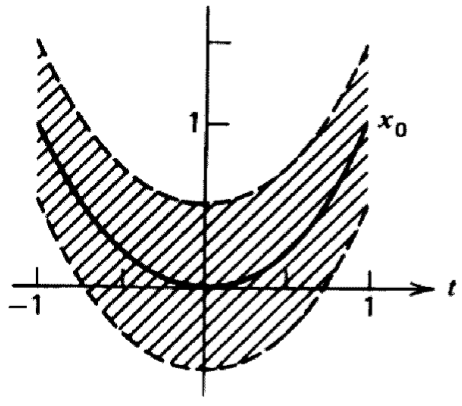
\includegraphics[width=0.5\textwidth]{kreyszig/assets/sec1-3-ex2.png}
    \caption{Region containing the graphs of all $x\in C[-1,1]$ which constitute the $\epsilon$-neighborhood, with $\epsilon=1/2$, of $x_0\in C[-1,1]$ given by $x_0(t)=t^2$.}
    \label{fig:fig1-3}
\end{figure}
\end{exercise}
\begin{proof}
$\R$: An open interval of the form $(a,b)$, where $b-a=2$ and the midpoint is $x_0$.

$\C$: If we think of $\C$ as $\R^2$ then it is a circle centered at $x_0$ with radius $1$, without the circumference of the circle.

$C[a,b]$: All the functions $g$ so that $\absoluteValue{g(t)-x_0(t)}<1$ for all $t$. 

We can see something similar in \Cref{fig:fig1-3}, where the shaded area is the area where the functions with $\absoluteValue{g(t)-t^2}<1/2$ can go through, for $t\in[-1,1]$.
\end{proof}

\begin{exercise}{3}
Consider $C[0,2\pi]$ and determine the smallest $r$ such that $y\in \hat{B}(x;r)$, where $x(t)=\sin t$ and $y(t)=\cos t$.
\end{exercise}
\begin{proof}
$r=1$ suffices, since the largest difference between $\sin t$ and $\cos t$ is 1 whenever $t=0$.
\end{proof}

\begin{exercise}{4}
Show that any nonempty set $A\subseteq (X,d)$ is open if and only if it is a union of open balls.
\end{exercise}
\begin{proof}
($\Rightarrow$) Suppose $A$ is open, then for every point in $x$ there is an open ball which is a subset of $A$. Thus $A$ is composed of open balls. That is, $A$ is a union of open balls.

($\Leftarrow$) Suppose $A$ is a union of open balls. Then any point in $x\in A$ belongs to one of these open balls, say $B(y;r)$. Let $r'=\min[d(x,y+r), d(x,y-r)]$, then $B(x;r')\subseteq B(y;r)\subseteq A$, so that there is an open ball around $x$ and $A$ is open.
\end{proof}

\begin{exercise}{5}
It is important to realise that certain sets may be open and closed at the same time. (a) Show that this is always the case for $X$ and $\emptyset$. (b) Show that in a discrete metric space $X$ (Cf. 1.1-8), every subset is open and closed.
\end{exercise}
\begin{proof}
(a) On page 19 Kreyszig proved that $\emptyset$ and $X$ are open. A set is closed if its complement is open. Hence given $X^C=\emptyset$ and $\emptyset^C=X$, both $X$ and $\emptyset$ are closed.

(b) From (a) we know that $X$ and $\emptyset$ are open and closed so let's consider a non trivial subset of $X$. Notice that every nonempty subset of $X$ is open, because for any $x\in X$, the set $\set{x}$ is a ball $B(x; r)$ for any $r<1$. But this means that the complement of any nonempty subset of $X$ is open because the same holds for any element of $X$. Hence, all subsets of $X$ are open and closed (clopen).
\end{proof}

\begin{exercise}{7}
Describe the closure of each of the following subsets. (a) The integers on $\R$, (b) the rational numbers on $\R$, (c) the complex numbers with rational real and imaginary parts in $\C$, (d) the disk $\set{z: \absoluteValue{z}<1}\subseteq\C$.
\end{exercise}
\begin{proof}
(a) Let $x\in\R$ and $x\notin\Z$. Notice that there are two integers $a,b$ so that $a<x<b$. Let $r=\min[x-a, b-x]$. We then have that $B(x,r)$ does not contain any element of $\Z$ and thus $x$ is not an accumulation point of $\Z$ in $\R$. As a result, $\Z=\overline{\Z}$ in $\R$.

(b) By the density of the rationals in the reals, any open ball around a rational contains an irrational number and hence it is an accumulation point. As a result, $\overline{\Q}=\R$.

(c) Following the same logic of (b), the closure of the complex numbers with rational real and imaginary parts is $\C$.

(d) This is similar to (b) and (c). Simply let $x\in\C$ have $\absoluteValue{x}=1$. For any $\epsilon>0$ we will always find that the ball $B(x;\epsilon)$ will contain an element of $\set{z: \absoluteValue{z}<1}$, so that $x\in\overline{\set{z: \absoluteValue{z}<1}}$. On the other hand, any number $y\in\C$ with $\absoluteValue{y}>1$ has an $\epsilon$-neighborhood so that no element of $\set{z: \absoluteValue{z}<1}$ belongs to it. Putting this together, we conclude that $\overline{\set{z: \absoluteValue{z}<1}}=\set{z: \absoluteValue{z}\leq 1}$.
\end{proof}

\begin{exercise}{8}
Show that the closure $\overline{B(x_0;r)}$ of an open ball $B(x_0;r)$ in a metric space can differ from the closed ball $\hat{B}(x_0;r)$.
\end{exercise}
\begin{proof}
Consider a set $X$ with the discrete metric. We have that $\hat{B}(x,1)=X$ for any $x\in X$. However, let $x,y\in X$ and consider the open ball $B(x;1)=\set{x}$. Think of the $\epsilon$-neighborhood around $y$ with $\epsilon=1/2$. Such $\epsilon$-neighborhood does not contain any element of $B(x;1)$, and so $y$ is not an accumulation point of $B(x;1)$. As a result, $B(x;1)=\overline{B(x;1)}\neq\hat{B}(x,1)=X$, as required.
\end{proof}

\begin{exercise}{9}
Show that 
\begin{enumerate}
    \item $A\subseteq\overline{A}$.
    \item $\overline{\overline{A}}=\overline{A}$.
    \item $\overline{A\cup B}=\overline{A}\cup\overline{B}$.
    \item $\overline{A\cap B}\subseteq\overline{A}\cap\overline{B}$.
\end{enumerate}
\end{exercise}
\begin{proof}
\begin{enumerate}
    \item By definition $\overline{A}$ contains $A$.
    \item We will prove this by double containment. $\overline{\overline{A}}\supseteq\overline{A}$ follows directly from the definition of closure. For the other direction, let $x\in \overline{\overline{A}}$. Then $x$ is either:
    
    (i) In $\overline{A}$, in which case $x\in\overline{\overline{A}}$ or,
    
    (ii) $x$ is an accumulation point of $\overline{A}$ not in $\overline{A}$.
    
    So suppose $x\notin \overline{A}$. Fix $\epsilon>0$, because $x$ is an accumulation point, there exists $y\in\overline{A}$ such that $d(x,y)\leq \epsilon/2$, and likewise because $y$ is in $A$ or it is one of its accumulation points, then  there exists $z\in A$ such that $d(y,z)\leq \epsilon/2$. Hence, $d(x,z)\leq d(x,y)+d(y,z) =\epsilon$ and so $x$ is an accumulation point of $A$ resulting in $x\in\overline{A}$. This contradicts (ii) so it must be the case that $x\in\overline{\overline{A}}$.
    \item We will prove this by double containment. 

    ($\subseteq$) Let $x\in\overline{A}\cup\overline{B}$. Then $x$ is either in $A$ or $B$ or an accumulation of either. If $x\in A$ or $x\in B$, then $x\in\overline{A}\cup\overline{B}$, so suppose $x\notin A,B$. Without loss of generality, suppose $x$ is an accumulation point of $A$. Then for every $\epsilon>0$, an open ball centered around $x$ with radius $\epsilon$ contains an element of $A$. But certainly it contains an element of $A\cup B$, so that $x\in\overline{A\cup B}$.

    ($\supseteq$) Let $x\in\overline{A\cup B}$. Then either $x\in A\cup B$ or $x$ is an accumulation of the union. In the former case, we would have that $x\in\overline{A}$ or $x\in\overline{B}$, so suppose that's not the case. Since $x$ is an accumulation point of $A\cup B$, then it must be the case there are infinite elements of $A\cup B$ that intersect open balls centered at $x$ (suppose this wasn't the case, then we could take the minimum of the distances between $x$ and every one of those elements of $A\cup B$, and then the open ball centered at $x$ with half such distance would not contain any element of $A\cup B$). However, this implies that there are either infinite elements of $A$ or infinite elements of $B$ that intersect open balls centered around $x$ (of any arbitrarily small radius), so that either $x\in\overline{A}$ or $x\in\overline{B}$.
    \item Suppose $x\in\overline{A\cap B}$, then either $x\in A\cap B$ or $x$ is an accumulation point of such set. If $x\in A\cap B$, then $x\in A$ and $x\in B$ so certainly $x\in\overline{A}\cap\overline{B}$ since $A\subseteq\overline{A}$ and $B\subseteq\overline{B}$. So suppose $x$ is an accumulation point of $A\cap B$. This implies that for every $\epsilon>0$, the open ball of radius $\epsilon$ centered at $x$ contains an element $y\in A\cap B$. Thus, for every $\epsilon>0$, there exists an element of $A$ such that it belongs to the open ball centered around $x$, so that $x\in\overline{A}$, following the same argument we can conclude that $x\in\overline{B}$ as well. That is, $x\in\overline{A}\cap\overline{B}$.
    \end{enumerate}
\end{proof}

\begin{exercise}{11 (Boundary)}
A boundary point $x$ of a set $A\subseteq (X,d)$ is a point of $X$ (which may or may not belong to $A$) such that every neighborhood of $x$ contains points of $A$ as well as points not belonging to $A$; and the boundary (or frontier) of $A$ is the set of all boundary points of $A$. Describe the boundary of (a) the intervals $(-1,1), [-1,1), [-1,1]$ on $\R$; (b) the set of all rational numbers on $\R$; (c) the disks $\set{z:\absoluteValue{z}<1}\subseteq\C$ and $\set{z:\absoluteValue{z}\leq 1}\subseteq\C$.
\end{exercise}
\begin{proof}
(a) For all intervals $-1$ and 1 are the boundary points. Simply consider for any $\epsilon>0$ the open ball around any of these two points. We will obtain than points in the intervals (and outside of them), are in such ball.

(b) Since the rationals are dense in $\R$, any open ball around any rational will contain both rationals and irrationals. Furthermore, for any irrational, we can find a rational that gets arbitrarily close to it. Hence, $\R$ is the boundary of $\R$.

(c) In both cases, the set $\set{z:\absoluteValue{z}=1}\subseteq\C$ is the boundary of the disks. That is because for any open ball around these points, we can find elements withing the disks and outside of them.
\end{proof}

\begin{exercise}{12 (Space $B[a,b]$)}
 Show that $B[a,b]$, $a<b$ is not separable (Cf. 1.2-2).
\end{exercise}
\begin{proof}
Suppose, for the sake of contradiction, that $B[a,b]$ is separable. Then there exists a countable set, call it $\FFF$, of functions so that for all functions in $g\in B[a,b]$, either $g\in\FFF$, or for all $\epsilon>0$, there exists a function $f\in\FFF$ with $f\in B(g;\epsilon)$.

Since $\FFF$ is countable we can find a bijection between $\FFF$ and $\N$, so that we can have a sequence of distinct numbers, $(x_n)$ where each $x_i\in[a,b]$ and $x_n$ can be mapped to a function, say $f_n\in\FFF$. Now let $h\in B[a,b]$ be defined as follows: for $h(x_n)=f_n(x_n)+1$ and 0 otherwise. We have that the open ball $B(h;1/2)$ does not contain any element of $\FFF$, so that $h$ is not an accumulation point of $\FFF$. Thus, $\overline{\FFF}\neq B[a,b]$ and $B[a,b]$ is not separable. 
\end{proof}

\begin{exercise}{13}
Show that a metric space $X$ is separable if and only if $X$ has a countable subset $Y$ with the following property. For every $\epsilon>0$ and every $x\in X$ there is a $y\in Y$ such that $d(x,y)<\epsilon$.
\end{exercise}
\begin{proof}
($\Rightarrow$) Suppose $X$ is separable. Then there exists a countable subset $Y\subseteq X$ so that $\overline{Y}=X$. But this means that for every $x\in X$, either $x\in Y$ or that for all $\epsilon>0$, there exists a $y\in Y$ with $y\in B(x, \epsilon)=\set{z\in X:d(x,z)<\epsilon}$, giving us the desired result.

($\Leftarrow$) Suppose there exists a countable subset $Y\subseteq X$ so that for every $\epsilon>0$, and every $x\in X$, there exists a $y\in Y$ with $d(x,y)<\epsilon$. Then this means that every $x\in X$ is an accumulation point, because for every $x$ and $\epsilon>0$ we can find $y\in Y$ with $y\in B(x,\epsilon)$. However, since all $x\in X$ are accumulation points of $Y$, then $\overline{Y}=X$, giving us that $X$ is separable, as required.
\end{proof}

\begin{exercise}{14 (Continuous mapping)} Show that a mapping $T:X\to Y$ is continuous if and only if the inverse image of any closed set $M\subseteq Y$ is a closed set in $X$.
\end{exercise}
\begin{proof}
Let $M$ be closed so that $M^C$ is open. By definition, we have that $(T^{-1}(M))^C=\set{x\in X:T(x)\notin M}=T^{-1}(M^C)$. 

For the ($\Rightarrow$) proof, if $T$ is continuous, then the inverse image of an open set is open, so that $T^{-1}(M^C)$ is open and by the equality above, then the inverse image of a closed set is closed. That is, $(T^{-1}(M))^C$ is open. 

For the converse, $(\Leftarrow)$, if the inverse image of a closed set is closed, so that $(T^{-1}(M))^C$ is open, by the equality above, we get that $T^{-1}(M^C)$ is open, so that the inverse image of an open set is open. That is, $T$ is continuous.
\end{proof}

\begin{exercise}{15}
Show that the image of an open set under a continuous mapping need not be open.
\end{exercise}
\begin{proof}
We have that $f:\R\to\R$ given by $f(x)=x^2$ is continuous. Consider the open set $A=(-1,1)\in\R$. We have that $f(A)=[0,1)$, which is not open in $\R$ because there is no open ball around 0 fully contained in $[0,1)$.
\end{proof}

\subsection{Convergence, Cauchy sequence, completeness}

\begin{exercise}{1 (Subsequence)}
If a sequence $(x_n)$ in a metric space $X$ is convergent and has limit $x$, show that every subsequence $(x_{n_k})$ of $(x_n)$ is convergent and has the same limit $x$.
\end{exercise}
\begin{proof}
Let $(x_{n_k})$ be a subsequence of $(x_n)$. Since $(x_n)$ converges to $x$, then for all $\epsilon>0$, there exists an $N\in\N$ so that for all $n>N$, it holds that $d(x_n,x)<\epsilon$. Fix $\epsilon>0$, and find $N\in\N$ as above. Now $N<n_K$ for some $K\in\N$, so that for all $k>K$ (and thus $n_k>N$, it holds that $d(x_{n_k},x)<\epsilon$ and $(x_{n_k})\to x$, as desired.
\end{proof}

\begin{exercise}{2}
If $(x_n)$ is Cauchy and has a convergent subsequence, say, $x_{n_k}\to x$, show that $(x_n)$ is convergent with the limit $x$.
\end{exercise}
\begin{proof}
Because $(x_n)$ is Cauchy, then for all $\epsilon>0$, there exists an $N\in\N$, so that for all $n,m>N$, it holds that $d(x_n,x_m)<\epsilon/2$. Likewise, there exists an $K\in\N$, so that for all $k>K$, it holds that $d(x_{n_K},x)<\epsilon/2$. Let $N'=\max[N,n_K]$, then for $n>N'$ and a fixed $n_k>N'$, we have $d(x_n,x)\leq d(x_n,x_{n_k})+d(x_{n_k},x)<\epsilon$
\end{proof}

\begin{exercise}{3}
Show that $x_n\to x$ if and only if for every neighborhood $V$ of $x$ there is an integer $n_0$ such that $x_n\in V$ for all $n>n_0$.
\end{exercise}
\begin{proof}
($\Rightarrow$) Suppose $x_n\to x$. Then for every $\epsilon>0$ there exists an $N$ so that for all $n>N$, it holds that $d(x_n,x)<\epsilon$. That is, no matter the size of the $\epsilon$-neighborhood inside $V$, we can find such $n_0$.

($\Leftarrow$) Suppose that for every neighborhood of $x$ we can find an $n_0$ so that for $n>n_0$ it holds that $x_n\in V$. Fix $\epsilon>0$ and let $V=B(x;\epsilon)$, then for $n>n_0$, it holds that $d(x_n,x)<\epsilon$. That is $x_n\to x$.
\end{proof}

\begin{exercise}{4 (Boundedness)}
Show that a Cauchy sequence is bounded.
\end{exercise}
\begin{proof}
A sequence is Cauchy if for all $\epsilon>0$, there exists an $N\in\N$ so that for all $n,m\geq N$, it holds that $d(x_n,x_m)<\epsilon$. Let $\delta=\max\set{d(x_N,x_k):k<N}$. We have that $\delta+\epsilon$ is a bound for the sequence because for arbitrary $x_n$ and $x_m$ in the sequence, $d(x_n,x_m)<\delta$ if $n,m<N$, $d(x_n,x_m)<\epsilon$ if $n,m\geq N$, and $d(x_n,x_m)\leq d(x_n,x_N)+d(x_N,x_m)=\delta+\epsilon$, if $n<N$ and $m\geq N$. 
\end{proof}

\begin{exercise}{5}
Is boundedness of a sequence in a metric space sufficient for the sequence to be Cauchy? Convergent?
\end{exercise}
\begin{proof}
Unfortunately no. Consider the real sequence (under the usual metric) given by $x_n=1$ if $n$ is even and $x_n=0$ if $n$ is odd. This sequence is pointwise bounded but certainly not Cauchy, nor convergent.
\end{proof}

\begin{exercise}{6}
If $(x_n)$ and $(y_n)$ are Cauchy sequences in a metric space $(X,d)$, show that $(a_n)$, where $a_n=d(x_n,y_n)$, converges. Give illustrative examples.
\end{exercise}
\begin{proof}
From exercise 1.1.12, we know that $\absoluteValue{d(x,y)-d(z,w)}\leq d(x,z)+d(y,w)$, so that $\absoluteValue{d(x_n,y_n)-d(x_m,y_m)}\leq d(x_n,x_m)+d(y_n,y_m)$. Fix $\epsilon>0$, since $(x_n)$ and $(y_n)$ are Cauchy, there exist $N,N'\in\N$, so that for all $n,m>N$ and $n',m'>N'$, it holds that $d(x_n,x_m)<\epsilon/2$ and $d(y_{n'},y_{m'})<\epsilon/2$. Let $M=\max[N,N']$, and $n,m>M$. We have $\absoluteValue{d(x_n,y_n)-d(x_m,y_m)}\leq d(x_n,x_m)+d(y_n,y_m)<\epsilon$, so that $(a_n)$ is Cauchy. Since $(a_n)$ is a Cauchy sequence in the reals, by the completeness of the reals (1.4-4), $(a_n)$ converges, as required.
\end{proof}

\begin{exercise}{8}
If $d_1$ and $d_2$ are metrics on the same set $X$ and there are positive numbers $a$ and $b$ such that for all $x,y\in X$, $ad_1(x,y)\leq d_2(x,y)\leq bd_1(x,y)$, show that the Cauchy sequences in $(X,d_1)$ and $(X,d_2)$ are the same.
\end{exercise}
\begin{proof}
Let $(x_n)$ be Cauchy in $(X,d_2)$. For $\epsilon>0$ there exists an $N\in\N$ such that for all $n,m>N$, it holds that $d_2(x_n,x_m)<\epsilon/a$, hence $d_1(x_n,x_m)<ad_2(x_n,x_m)<a\epsilon/a=\epsilon$ and $(x_n)$ is also Cauchy in $(X,d_1)$. We can prove that a Cauchy sequence in $(X,d_1)$ is Cauchy in $(X,d_2)$ mutatis mutandis.
\end{proof}

\begin{exercise}{9}
Using exercise 8, show that the metric space in exercises 13 to 15 of Section 1.2 have the same Cauchy sequences.
\end{exercise}
\begin{proof}
We have that 
\[
\max[d_1(x_1,y_1),d_2(x_2,y_2)]
\leq d_1(x_1,y_1)+d_2(x_2,y_2)
\leq 2\max[d_1(x_1,y_1),d_2(x_2,y_2)],
\]
so that $\bar{d}(x,y)$ and $d(x,y)$ are equivalent.

Furthermore,
\[
\max[d_1(x_1,y_1),d_2(x_2,y_2)]
\leq \sqrt{d_1(x_1,y_1)^2+d_2(x_2,y_2)^2}
\leq \sqrt{2}\max[d_1(x_1,y_1),d_2(x_2,y_2)],
\]
so that $\bar{d}(x,y)$ and $\hat{d}(x,y)$ are equivalent.

Since being equivalent in this sense is an equivalence relation, then $d(x,y)$ and $\hat{d}(x,y)$ are equivalent, as required.
\end{proof}

\begin{exercise}{10}
Using the completeness of $\R$, prove the completeness of $\C$.
\end{exercise}
\begin{proof}
Let $(x_n)$ be a Cauchy sequence in $\C$. That is, $x_n$ can be written as $a_n+ib_n$ for $a_n,b_n\in\R$. Let $\epsilon>0$, then we can find $N\in\N$ so that for any $n,m>N$, we have that $d(x_n,x_m)=\sqrt{(a_n-a_m)^2+(b_n-b_m)^2}<\epsilon$. 

From the previous statement, we can see that for the same $n$ and $m$, it holds that $d(a_n,a_m)\leq \epsilon$ and $d(b_n,b_m)\leq \epsilon$ under the euclidean metric. That is, $(a_n)$ and $(b_n)$ are Cauchy. Since they are Cauchy, they converge to say $a$ and $b$ so that $x_n$ converges to $a+ib$, as required.
\end{proof}
\subsection{Examples. Completeness proofs}

\begin{exercise}{1}
fill
\end{exercise}
\begin{proof}
fill
\end{proof}
\subsection{Completion of metric spaces}

\begin{exercise}{1}
fill
\end{exercise}
\begin{proof}
fill
\end{proof}

\section{Normed spaces. Banach spaces}
\subsection{Vector space}

\begin{exercise}{1}
fill
\end{exercise}
\begin{proof}
fill
\end{proof}
\subsection{Normed space. Banach space}

\begin{exercise}{1}
fill
\end{exercise}
\begin{proof}
fill
\end{proof}
\subsection{Further properties of normed spaces}

\begin{exercise}{1}
fill
\end{exercise}
\begin{proof}
fill
\end{proof}
\subsection{Finite dimensional normed spaces and subspaces}

\begin{exercise}{1}
fill
\end{exercise}
\begin{proof}
fill
\end{proof}
\subsection{Compactness and finite dimension}

\begin{exercise}{1}
fill
\end{exercise}
\begin{proof}
fill
\end{proof}
\subsection{Linear operators}

\begin{exercise}{1}
fill
\end{exercise}
\begin{proof}
fill
\end{proof}
\subsection{Bounded and continuous linear operators}

\begin{exercise}{1}
fill
\end{exercise}
\begin{proof}
fill
\end{proof}
\subsection{Linear functionals}

\begin{exercise}{1}
fill
\end{exercise}
\begin{proof}
fill
\end{proof}
\subsection{Linear operators and functional on finite dimensional spaces}

\begin{exercise}{1}
fill
\end{exercise}
\begin{proof}
fill
\end{proof}
\subsection{Normed spaces of operators. Dual space}

\begin{exercise}{1}
fill
\end{exercise}
\begin{proof}
fill
\end{proof}

\section{Inner product spaces. Hilbert spaces}
\subsection{Inner product space. Hilbert space}

\begin{exercise}{1}
fill
\end{exercise}
\begin{proof}
fill
\end{proof}

\section{Fundamental theorems for normed and Banach spaces}
\subsection{Zorn's Lemma}

\begin{exercise}{1}
fill
\end{exercise}
\begin{proof}
fill
\end{proof}

\section{Further applications: Banach fixed point Theorem}
\subsection{Banach fixed point Theorem}

\begin{exercise}{1}
fill
\end{exercise}
\begin{proof}
fill
\end{proof}

\section{Further applications: approximation theory}
\subsection{Approximation in normed spaces}

\begin{exercise}{1}
fill
\end{exercise}
\begin{proof}
fill
\end{proof}

\section{Spectral theory of linear operators in normed spaces}
\subsection{Spectral theory in finite dimensional normed spaces}

\begin{exercise}{1}
fill
\end{exercise}
\begin{proof}
fill
\end{proof}

\section{Compact linear operators on normed spaces and their spectrum}
\subsection{Compact linear operators on normed spaces}

\begin{exercise}{1}
fill
\end{exercise}
\begin{proof}
fill
\end{proof}

\section{Spectral theory of bounded self-adjoint linear operators}
\subsection{Spectral properties of bounded self-adjoint linear operators}

\begin{exercise}{1}
fill
\end{exercise}
\begin{proof}
fill
\end{proof}

\section{Unbounded linear operators in Hilbert space}
\subsection{Unbounded linear operators and their Hilbert-adjoint operators}

\begin{exercise}{1}
fill
\end{exercise}
\begin{proof}
fill
\end{proof}

\section{Unbounded linear operators in quantum mechanics}
\subsection{Basic ideas. States. Observables, position operator}

\begin{exercise}{1}
fill
\end{exercise}
\begin{proof}
fill
\end{proof}

\end{document}